\documentclass{beamer}
\usetheme{Warsaw}
\usepackage[utf8]{inputenc}
\usepackage[ngerman]{babel}

\title{Monitoringsystem einer Ambient Assisted Living-Anwendung mit Hilfe der eXist Datenbank}
\author{Adam Kucera, Andre Krause, Robert Riedel}
\date{\today}

\begin{document}
\maketitle
\begin{frame}
	\frametitle{Inhalt}
	\tableofcontents[%
% 		currentsection, % causes all sections but the current to be shown in a semi-transparent way.
% 		currentsubsection, % causes all subsections but the current subsection in the current section to ...
% 		hideallsubsections, % causes all subsections to be hidden.
 		hideothersubsections, % causes the subsections of sections other than the current one to be hidden.
% 		part=, % part number causes the table of contents of part part number to be shown
%		pausesections, % causes a \pause command to be issued before each section. This is useful if you
% 		pausesubsections, %  causes a \pause command to be issued before each subsection.
% 		sections={ overlay specification },
	]
\end{frame}

\section{Problemstellung}
\begin{frame}
\frametitle{Problemstellung}
\begin{itemize}
	\item Anteil älterer Menschen nimmt zu
	\item Betreuung in eigenen vier Wänden schwierig
	\item Möglichkeit muss gefunden werden, dies zu ermöglichen
	\item Einsatz technischer Hilfsmittel
	%\item Ambient Assisted Living (AAL) = 
\end{itemize}
\begin{Definition}
Ambient Assisted Living (AAL) ist die Vernetzung des Wohnraums an sich und mit externen Dienstleistern zur alltäglichen Unterstützung und Überwachung.
\end{Definition}
\end{frame}

\section{Aufgabenstellung}
\begin{frame}
\frametitle{Aufgabenstellung}
\begin{itemize}
	\item Überwachung der Vitalwerte durch Sensoren
	\item In Wänden oder am Handgelenk
	\item Senden Werte an zentrale Stelle
	\item In Datenbank abgespeichert
	\item An Monitoring System weitergeleitet
\end{itemize}
\end{frame}

\begin{frame}
\frametitle{Aufgabenstellung}
\begin{itemize}
	\item Erstellen einer Server-Client Anwendung mit Hilfe von XML-Technologien
	\item eXist als Datenbank
	\item Webclient zur Anzeige der Vitalwerte
	\item Reporterstellung
\end{itemize}
\end{frame}

\section{Entwurf}
\begin{frame}
\frametitle{Use-Cases}
\end{frame}

\begin{frame}
\frametitle{Technologien}
\begin{itemize}
	\item eXist
	\item HTML5+Javascript
	\item Node.JS
	\item XML
	\item XQuery
	\item XSLT - XSL-FO - PDF
	\item REST
	\item Websockets
\end{itemize}
\end{frame}

\begin{frame}
\frametitle{System-Architektur}
\begin{figure}[H]
\begin{center}
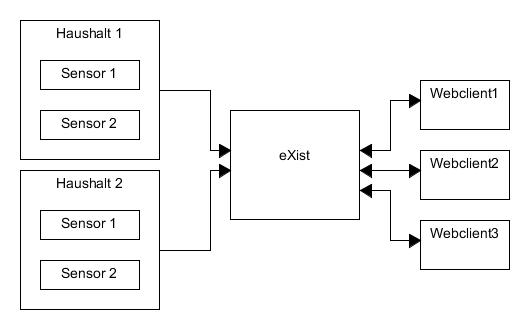
\includegraphics[scale=0.5]{images/sa1.jpg} 
\end{center}
\end{figure}
\end{frame}

\begin{frame}
\frametitle{System-Architektur}
\begin{figure}[H]
\begin{center}
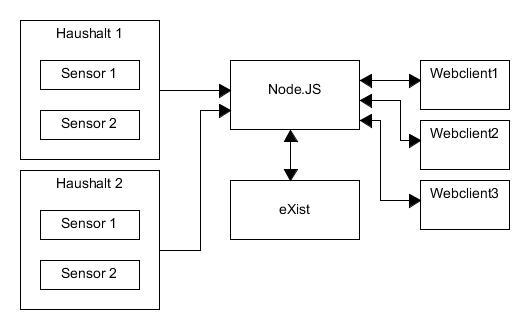
\includegraphics[scale=0.5]{images/sa2.jpg} 
\end{center}
\end{figure}
\end{frame}

\begin{frame}
\frametitle{Kommunikation}
\end{frame}

\end{document}